\def\theTopic{Reading 3}


\section{ Ethical Instincts of Babies?}


Researchers at Yale University were interested in how soon in human
development children become aware of (and start to favor) activities
that help rather than hinder others.\\
Title: ``Social evaluation by preverbal infants''
\\
Authors: J. Kiley Hamlin, Karen Wynn \& Paul Bloom
\\
Journal: {\it Nature} 450, 557-559 (22 November 2007) 
\\
Abstract \vspace{-.5cm}
\begin{quotation}
  The capacity to evaluate other people is essential for navigating the
social world. Humans must be able to assess the actions and intentions
of the people around them, and make accurate decisions about who is
friend and who is foe, who is an appropriate social partner and who is
not. Indeed, all social animals benefit from the capacity to identify
individuals  that may help them, and to distinguish these
individuals from others that may harm them. Human adults evaluate
people rapidly and automatically on the basis of both behavior and
physical features, but the origins and
development of this capacity are not well understood. Here we show
that 6- and 10-month-old infants take into account an individual's
actions towards others in evaluating that individual as appealing or
aversive: infants prefer an individual who helps another to one who
hinders another, prefer a helping individual to a neutral individual,
and prefer a neutral individual to a hindering individual. These
findings constitute evidence that preverbal infants assess individuals
on the basis of their behavior towards others. This capacity may
serve as the foundation for moral thought and action, and its early
developmental emergence supports the view that social evaluation is a
biological adaptation. 



The following were randomized across subjects:
(1) color/shape of helper and hinderer; (2) order of helping and
hindering events; (3) order of choice and looking time
measures; and (4) positions of helper and hinderer. 
\end{quotation}

\begin{center}
        {\large\bf Strength of Evidence}
 \end{center}
      The observed result gets compared to the distribution from the
      simulation to gauge the evidence against $H_0$.  That's
      how the scientific method works.  We formulate a hypothesis
      which can be falsified, then see if the data collected argue
      against the hypothesis. Sometimes our result provides a lot of
      evidence against the null model  -- when the observed result is very
      unlikely -- while other times it has very little evidence against
      the null model -- when the observed result is likely under the null
      model. To explain to others  how likely or unlikely the
      observed result is under the null model, we  report the
      ``strength of evidence'' -- also called  the p-value.

       {\bf Definition:} The p-value is the probability of observing a
       results at least as the result we have observed if the null
       hypothesis is true. 
 
       We quantify the strength of evidence by answering the question:
       ``If $H_0$ is true, what proportion of the simulated results
       are as unusual as (or even more unusual than) the observed
       result?''  For example, consider the results from ``Martian
       Alphabet'' in Figure 1. A group of 12 humans had 9 correct
       matches and 3 incorrect. The simulation assumed $H_0: p = 0.5$,
       and counted the number of heads in 12 flips of a fair
       coin. (Head $\leftrightarrow$ Correct).  The whole process was
       simulated 1000 times and the number of outcomes at 9 or above
       on the plot are those as extreme or more extreme as the group's
       score. The chance is 74/1000 = 0.074 of getting a result this
       extreme when $H_0$ is true.  The p-value of 0.074 is the
       strength of evidence against $H_0$ for 9 correct matches. It is
       the probability of obtaining results as extreme or more extreme
       when $H_0$ true. 

 \begin{figure}[h]
   \centering
  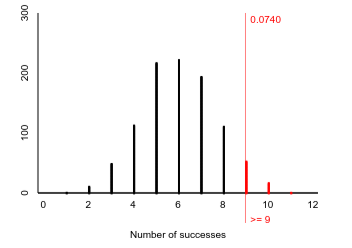
\includegraphics[width=.5\linewidth]{../plots/StrOfEvidence-12Guesses.png}

   \caption{ Simulation results obtained from the null model. The
      outcomes 9 and higher (74 out of 1000 trials) were as or more extreme
      as one group's number correct (of 12) and indicate the strength of
      evidence $=$ 0.074. }
   \label{fig:SOE-12}
 \end{figure}
  For this group of 12, we would say that there is some evidence that
  they can read Martian, but while an  event which can happen  7\% of
  the time is   fairly rare, it may not be totally convincing.  
  A p-value  of 0.07 is not really tiny, but is  a ``cautionary'' yellow
  light. 

 \begin{center}
   {\large\bf Important Points}
 \end{center}
 \begin{itemize}
 \item From the abstract, what was the research question?\vspace{1cm}
 \item What response was recorded? What type of variable is the
   response? \vspace{1cm}
 \item How was randomness utilized?\vspace{1cm}
 \item Would an outcome of 10 or of 8 provide stronger evidence
   against the null than our observed outcome of 9?\vfill
 \item Do smaller or larger p-values provide strong evidence against
   the null hypothesis? 
 \end{itemize}



